%%%%%%%%%%%%%%%%%%%%%%%%%%%%%%%%%%%%%%%%%
% Sullivan Business Report
% LaTeX Template
% Version 1.0 (May 5, 2022)
%
% This template originates from:
% https://www.LaTeXTemplates.com
%
% Author:
% Vel (vel@latextemplates.com)
%
% License:
% CC BY-NC-SA 4.0 (https://creativecommons.org/licenses/by-nc-sa/4.0/)
%
%%%%%%%%%%%%%%%%%%%%%%%%%%%%%%%%%%%%%%%%%


%----------------------------------------------------------------------------------------
%	CLASS, PACKAGES AND OTHER DOCUMENT CONFIGURATIONS
%----------------------------------------------------------------------------------------

\documentclass[
    a4paper, % Paper size, use either a4paper or letterpaper
	12pt, % Default font size, the template is designed to look good at 12pt so it's best not to change this
	%unnumberedsections, % Uncomment for no section numbering
    ]{CSSullivanBusinessReport}
    
    \addbibresource{sample.bib} % BibLaTeX bibliography file

%----------------------------------------------------------------------------------------
%	REPORT INFORMATION
%----------------------------------------------------------------------------------------

\reporttitle{CPE 233 Hardware Assignment 2} % The report title is to appear on the title page and page headers, do not create manual new lines here as this will carry over to page headers

\reportsubtitle{Program Counter and Verification} % Report subtitle, include new lines if needed

\reportauthors{Report by:\\\smallskip Ethan Vosburg (evosburg@calpoly.edu)} % Report authors/group/department, include new lines if needed

\reportdate{\today} % Report date, include new lines for additional information if needed

\rightheadercontent{
\includegraphics[width=3cm]{creodocs_logo.pdf}} % The content in the right header, you may want to add your own company logo or use your company/department name or leave this command empty for no right header content

%----------------------------------------------------------------------------------------

\begin{document}

%----------------------------------------------------------------------------------------
%	TITLE PAGE
%----------------------------------------------------------------------------------------

\thispagestyle{empty} % Suppress headers and footers on this page

\begin{fullwidth} % Use the whole page width
	\vspace*{-0.075\textheight} % Pull logo into the top margin
	
	\hfill
\includegraphics[width=5cm]{creodocs_logo.pdf} % Company logo

	\vspace{0.15\textheight} % Vertical whitespace

	\parbox{0.9\fulltextwidth}{\fontsize{50pt}{52pt}\selectfont\raggedright\textbf{\reporttitle}\par} % Report title, intentionally at less than full width for nice wrapping. Adjust the width of the \parbox and the font size as needed for your title to look good.
	
	\vspace{0.03\textheight} % Vertical whitespace
	
	{\LARGE\textit{\textbf{\reportsubtitle}}\par} % Subtitle
	
	\vfill % Vertical whitespace
	
	{\Large\reportauthors\par} % Report authors, group or department
	
	\vfill\vfill\vfill % Vertical whitespace
	
	{\large\reportdate\par} % Report date
\end{fullwidth}

\newpage

%----------------------------------------------------------------------------------------
%	DISCLAIMER/COPYRIGHT PAGE
%----------------------------------------------------------------------------------------

% \thispagestyle{empty} % Suppress headers and footers on this page

% \begin{twothirdswidth} % Content in this environment to be at two-thirds of the whole page width
% 	\footnotesize % Reduce font size
	
% 	\subsection*{Disclaimer}

% 	Lorem ipsum dolor sit amet, consectetur adipiscing elit. Praesent porttitor arcu luctus, imperdiet urna iaculis, mattis eros. Pellentesque iaculis odio vel nisl ullamcorper, nec faucibus ipsum molestie. Sed dictum nisl non aliquet porttitor. Etiam vulputate arcu dignissim, finibus sem et, viverra nisl. Aenean luctus congue massa, ut laoreet metus ornare in. Nunc fermentum nisi imperdiet lectus tincidunt vestibulum at ac elit.
	
% 	\subsection*{Copyright}
	
% 	\textcopyright~[Year] [Company] 
	
% 	Copyright notice text\ldots In hac habitasse platea dictumst. Curabitur mattis elit sit amet justo luctus vestibulum. In hac habitasse platea dictumst. Pellentesque lobortis justo enim, a condimentum massa tempor eu. Ut quis nulla a quam pretium eleifend nec eu nisl. Nam cursus porttitor eros, sed luctus ligula convallis quis.
	
% 	\subsection*{Contact}
	
% 	Address Line 1\\
% 	Address Line 2\\
% 	Address Line 3
	
% 	Business Number 123456
	
% 	Contact: name@company.com
	
% 	\vfill % Push the following down to the bottom of the page
	
% 	\subsubsection*{Changelog}
	
% 	\scriptsize % Reduce font size further
	
% 	\begin{tabular}{@{} L{0.05\linewidth} L{0.15\linewidth} L{0.6\linewidth} @{}} % Column widths specified here, change as needed for your content
% 		\toprule
% 		v1.0 & 20XX-02-05 & Lorem ipsum dolor sit amet, consectetur adipiscing elit. Praesent porttitor arcu luctus, imperdiet urna iaculis, mattis eros.\\
% 		v1.1 & 20XX-02-27 & Pellentesque iaculis odio vel nisl ullamcorper, nec faucibus ipsum molestie.\\
% 		v1.2 & 20XX-03-15 & Sed dictum nisl non aliquet porttitor.\\
% 		\bottomrule
% 	\end{tabular}
% \end{twothirdswidth}

% \newpage

%----------------------------------------------------------------------------------------
%	TABLE OF CONTENTS
%----------------------------------------------------------------------------------------
\bigskip
\begin{twothirdswidth} % Content in this environment to be at two-thirds of the whole page width
	\tableofcontents % Output the table of contents, automatically generated from the section commands used in the document
\end{twothirdswidth}

\newpage

%----------------------------------------------------------------------------------------
%	SECTIONS
%----------------------------------------------------------------------------------------
\begin{fullwidth} % Use the whole page width

\section{Project Description} % Top level section

In this project, a program counter for the Otter processor was created. The program counter is a register that holds the address of the next instruction to be executed. The program counter is incremented by 4 every clock cycle. The program counter is also able to be reset to 0. The program counter was then tested using a testbench. The testbench went through several test cases to verify that the program counter and the mux associated with it work properly. The testbench was able to be run and passed all of the test cases.


\section{Structural Design} % Second level section

\subsection{Overall Elaborated Design} % Third level section

\begin{figure}[H]
    \centering
    \captionsetup{style=widetable}
    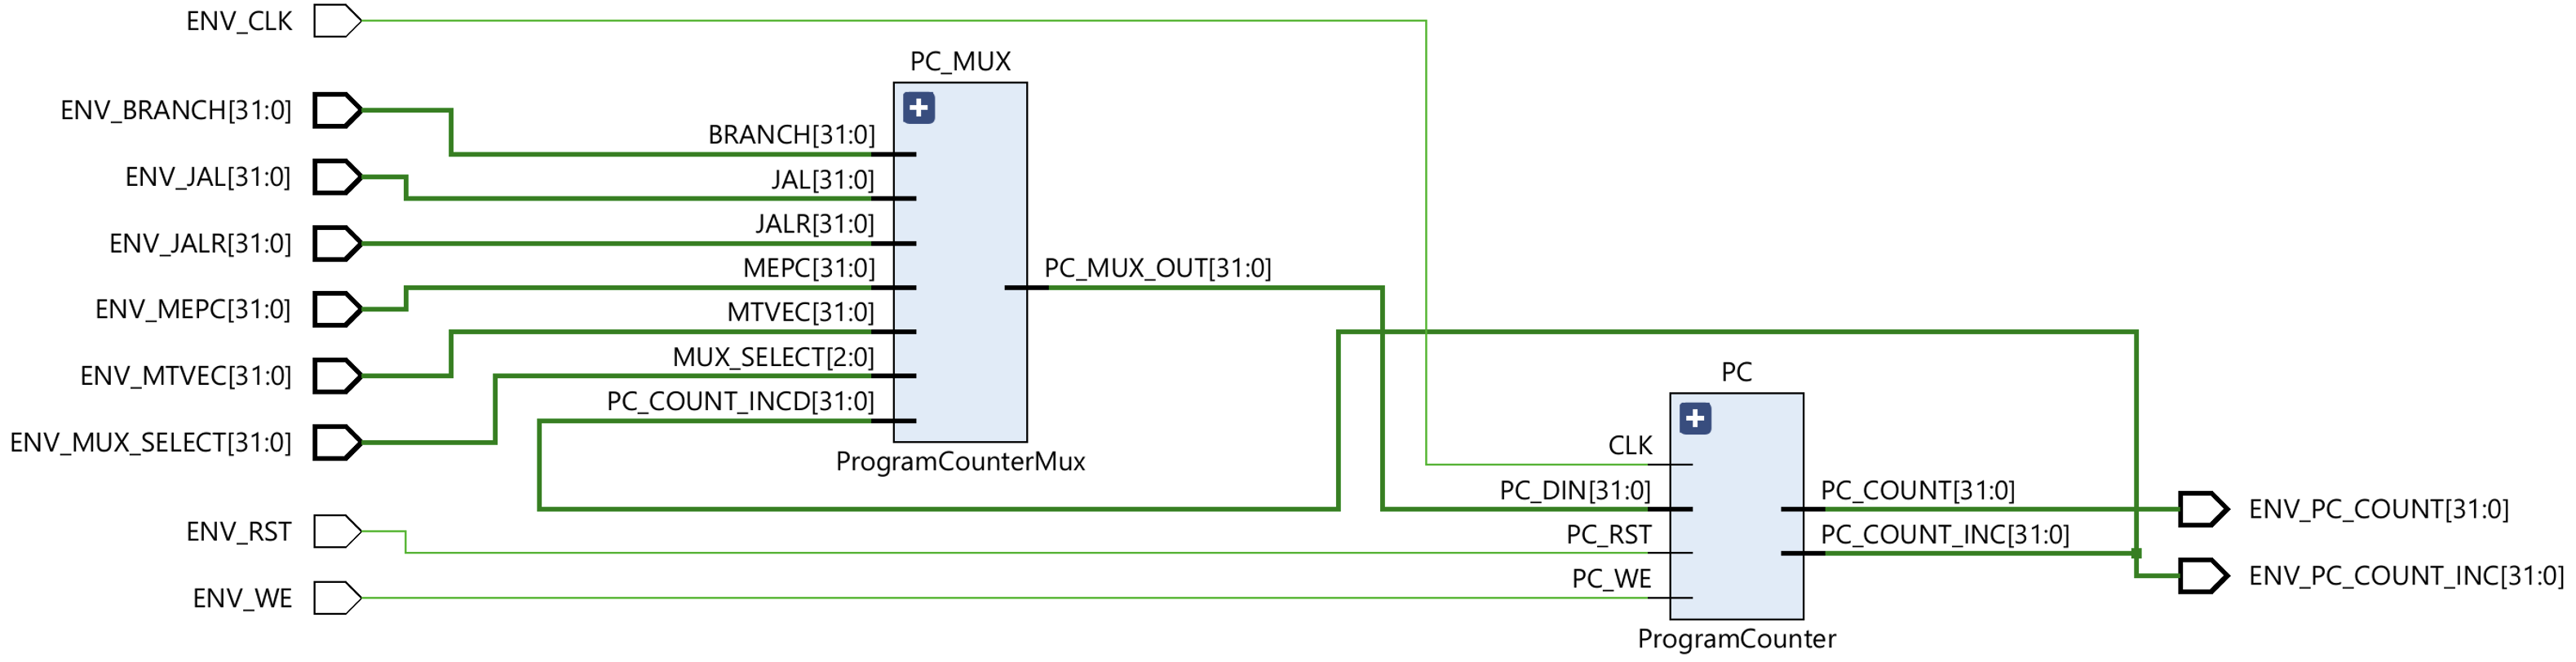
\includegraphics[width=.80\pdfpagewidth]{Figures/Program Counter Elaborated Design.png}
    \caption{Program Counter Elaborated Design}
    \label{fig:PCElaboratedDesign}
\end{figure}

\subsection{Program Counter Multiplexer Elaborated Design} % Third level section

\begin{figure}[H]
    \captionsetup{style=widetable}
    \makebox[.80\pdfpagewidth]{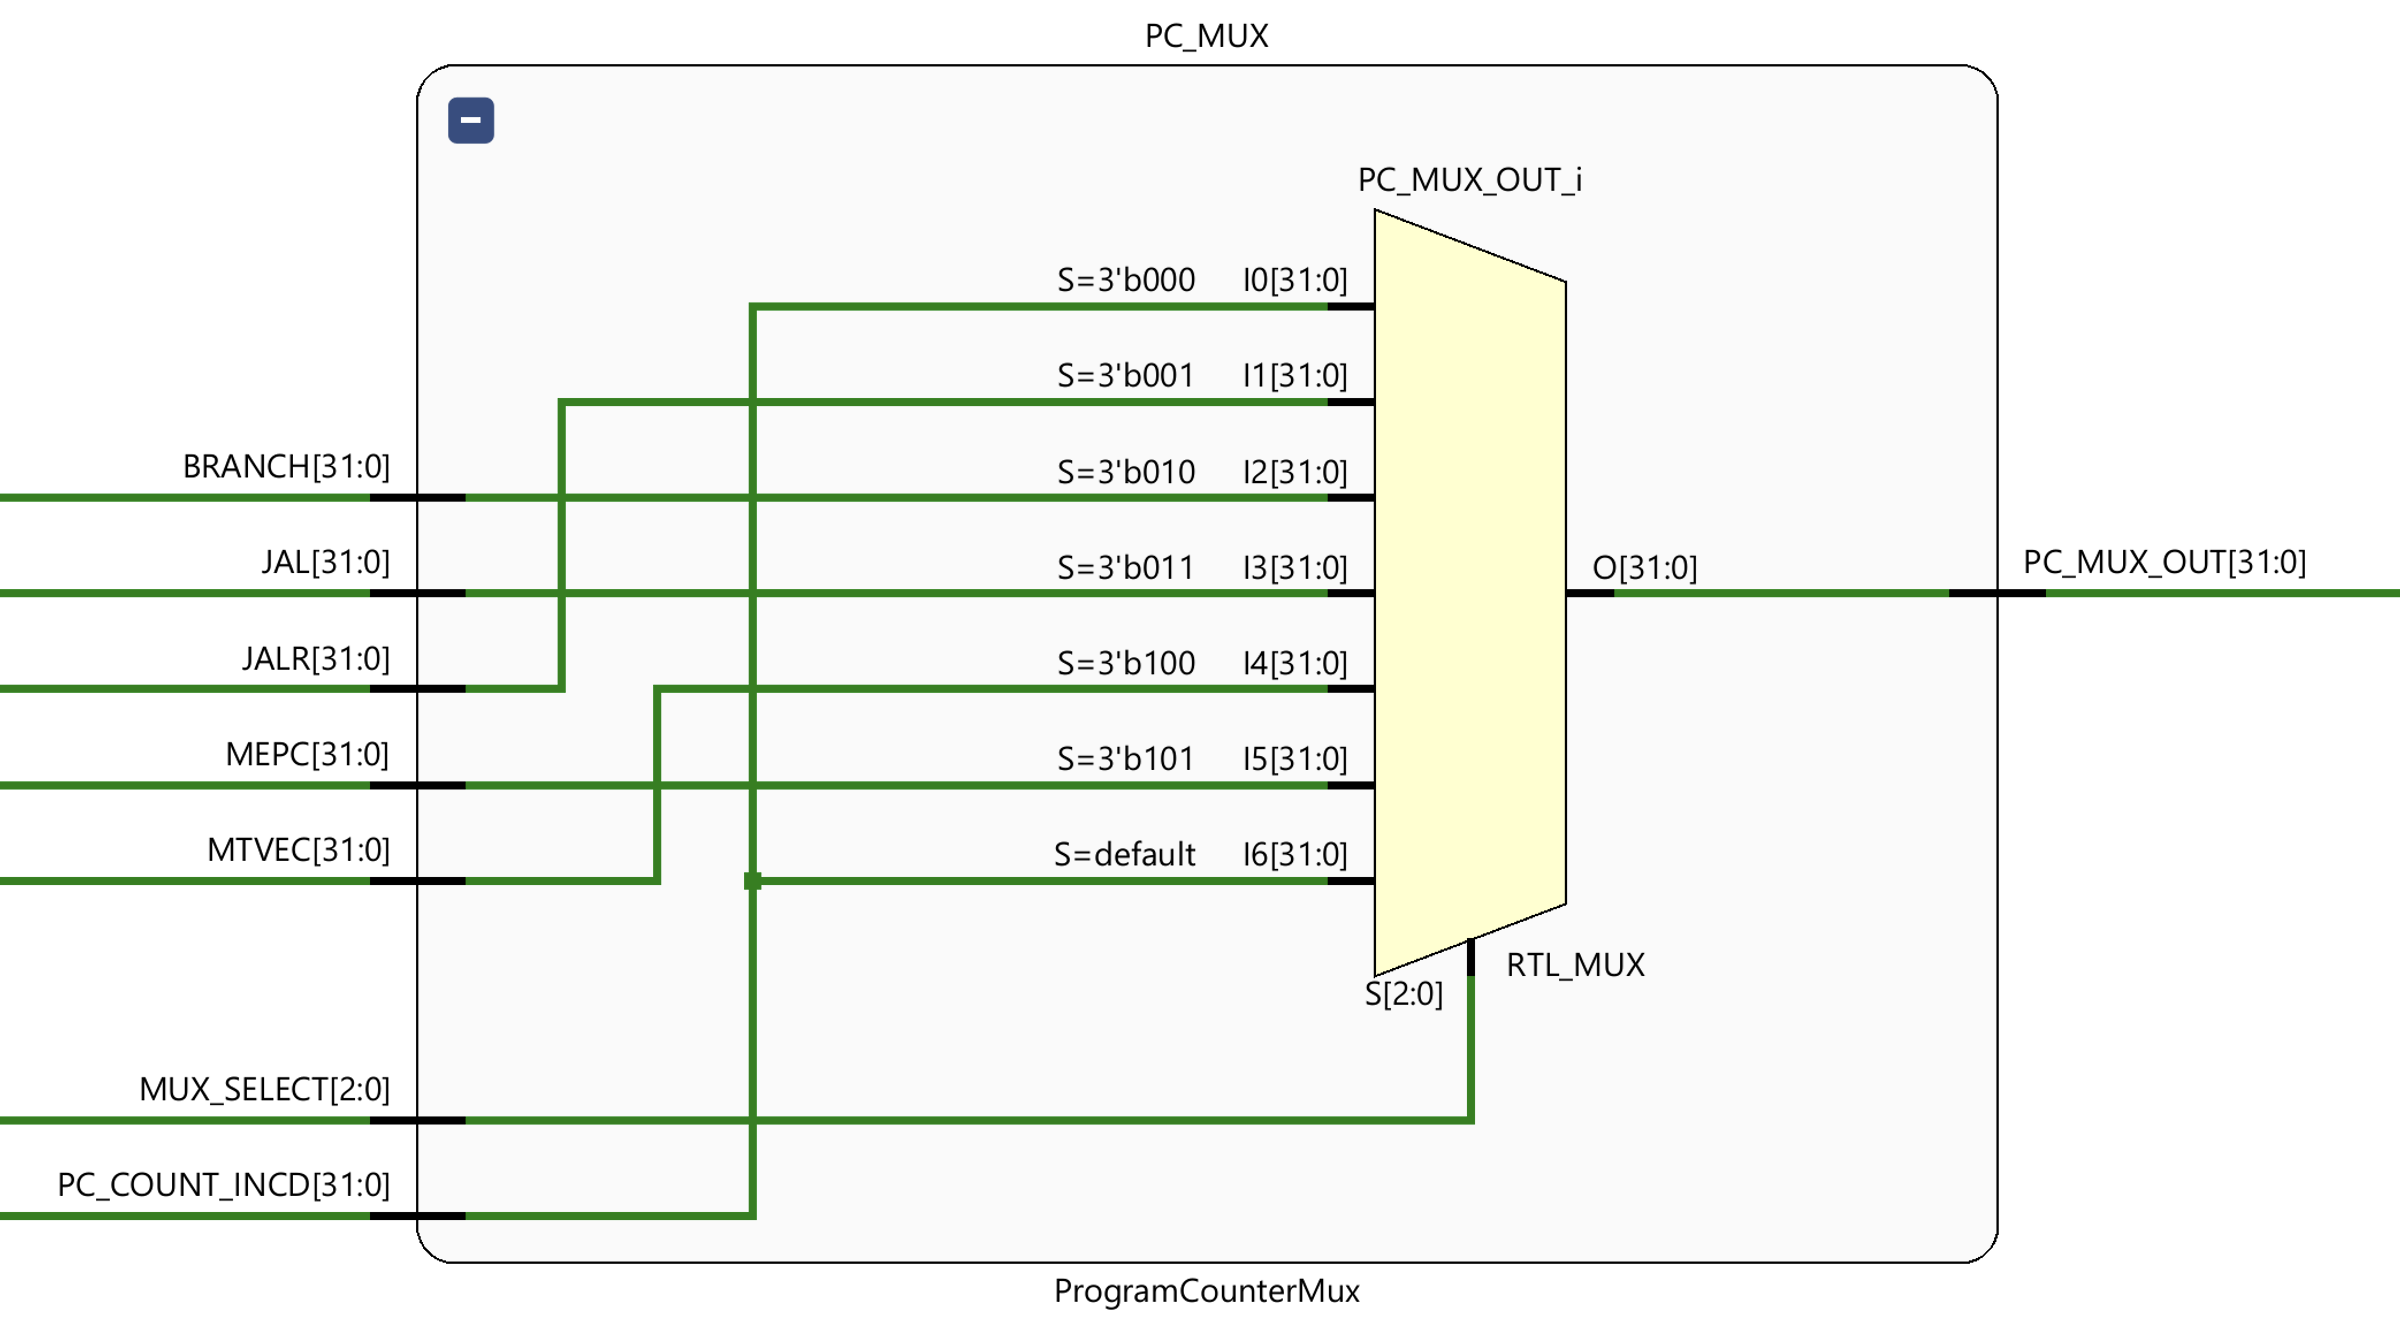
\includegraphics[width=.5\pdfpagewidth]{Figures/Program Counter Mux.png}}
    \caption{Program Counter Multiplexer Elaborated Design}
    \label{fig:PCMUXElaboratedDesign}
\end{figure}

\subsection{Program Counter Main Hardware Elaborated Design} % Third level section

\begin{figure}[H]
    \makebox[.80\pdfpagewidth]{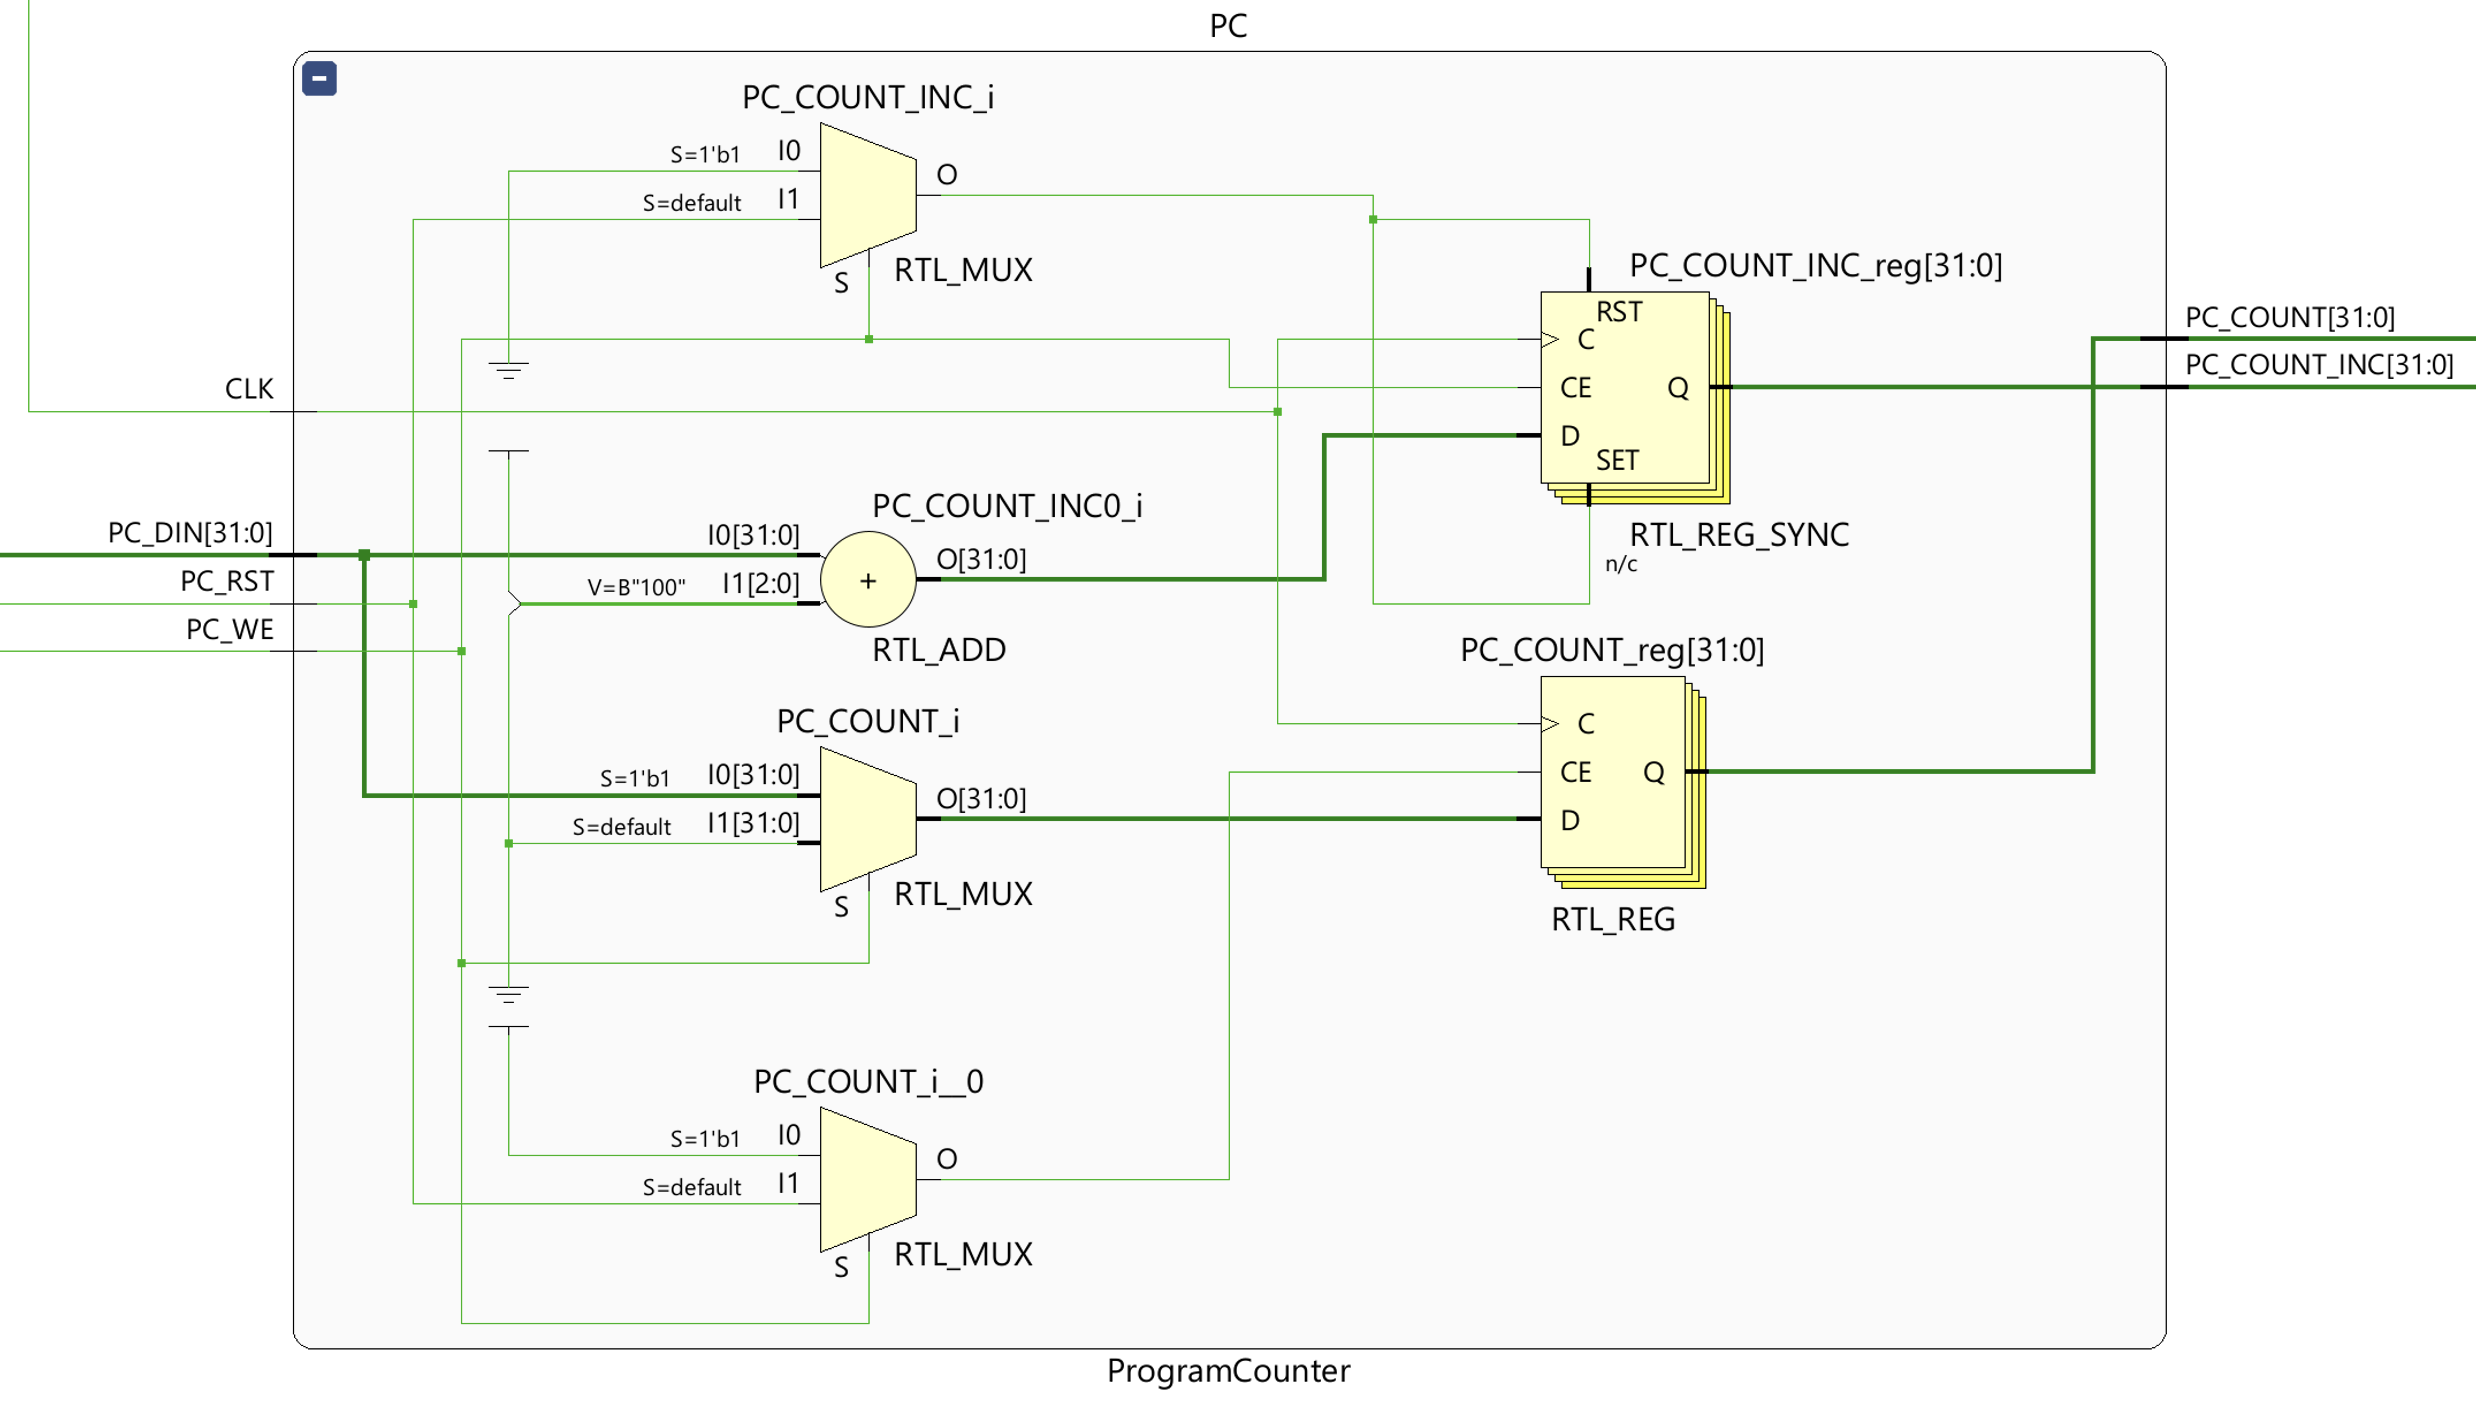
\includegraphics[width=.5\pdfpagewidth]{Figures/Program Counter Main Hardware.png}}
    \caption{Program Counter Main Hardware Elaborated Design}
    \label{fig:PCMainHardwareElaboratedDesign}
\end{figure}

\section{Synthesis Warnings Listing} % Second level section

\begin{figure}[H]
    \captionsetup{style=widetable}
    \makebox[.80\pdfpagewidth]{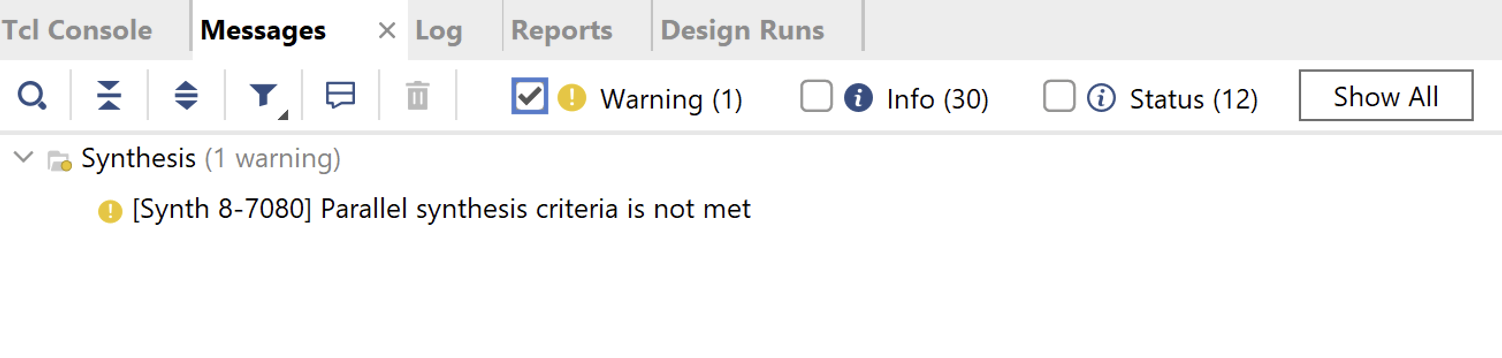
\includegraphics[width=.75\pdfpagewidth]{Figures/Program Counter Console Warnings.png}}
    \caption{Synthesis Warnings}
    \label{fig:SynthesisWarnings}
\end{figure}

\section{Verification} % Second level section

\subsection{Testbench Coverage} % Third level section

When testing this design, there were several test cases that were used to verify that the design was working properly. The test cases are listed below.

\begin{enumerate}
    \item \textbf{ReadMux Test:} This test checks that the mux can read all Inputs properly. The testbench sets the different inputs of the mux to 10 times the select value and then checks that the output is equal to the select value.
    \item \textbf{MaxMux Test:} This test checks that when the maximum 32-bit value of the program counter is reached, the failure is predictable and expected.
    \item \textbf{MinMux Test:} This test checks that when the minimum 32-bit value is loaded into all of the inputs, only valid next addresses are outputted.
    \item \textbf{Reset Test:} This test checks that the reset is working properly. The testbench sets the reset to 1 and then checks that the output of the program counter is 0.
    \item \textbf{RandNum Test:} This test checks that when random numbers are inputted into the program counter, the output is predictable and expected. 
    \item \textbf{WriteEnable Test:} This test checks that the write enable is working properly. When the write enable is set to 0, the program counter should not change. When the write enable is set to 1, the program counter should increment by 4.
\end{enumerate}

\subsection{Testbench Code} % Third level section

\begin{lstlisting}[language=Verilog, caption=Verilog Testbench for Program Counter]{/Users/ethanvosburg/Documents/git/CPE-233-Otter/HW2-ProgramCounter/ProgramCounter/ProgramCounter.srcs/sim_1/new/ProgramCounterEnv_TB.sv}

\subsection{Testbench Output} % Third level section
Here is the output from the console after running this testbench.

\begin{lstlisting}[language=Verilog, caption=TCl Output from ProgramCounterEnv\_TB]
    Setup Complete
    ReadMux Test Passed
    MaxMux Test Passed
    MinMux Test Passed
    Reset Test Passed
    RandNum Test Passed
    WriteEnable Test Passed
    All Tests Passed
    $finish called at time : 300 ns
\end{lstlisting}

Running this testbench results in this simulation wavefrom.

\begin{figure}[H]
    \centering
    \captionsetup{style=widetable}
    \makebox[.80\pdfpagewidth]{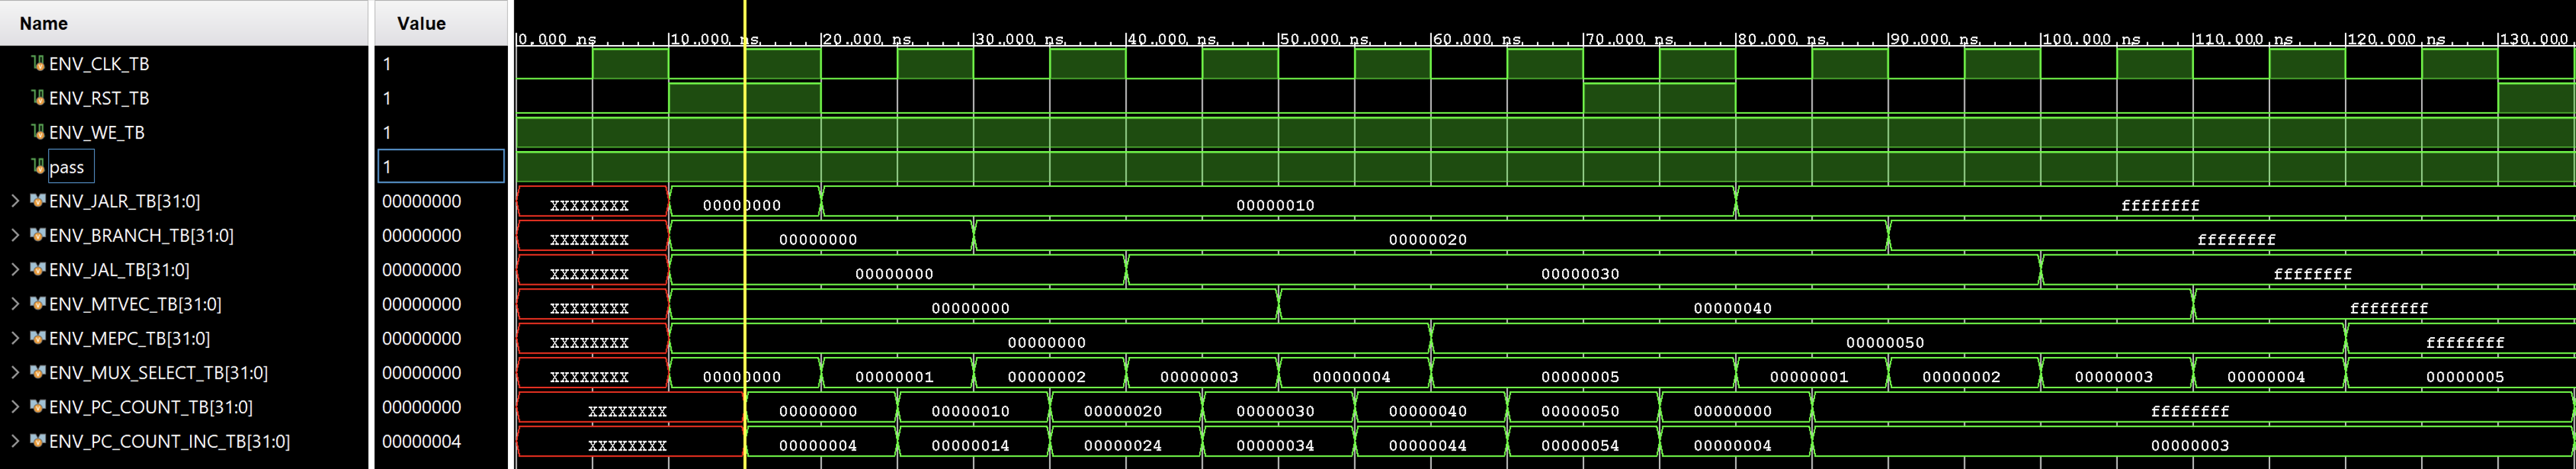
\includegraphics[width=.8\pdfpagewidth]{Figures/Program Counter Simulation 1.png}}
    \caption{Program Counter Simulation 0ns - 130ns}
    \label{fig:PCSimulation}
\end{figure}

\begin{figure}[H]
    \centering
    \captionsetup{style=widetable}
    \makebox[.80\pdfpagewidth]{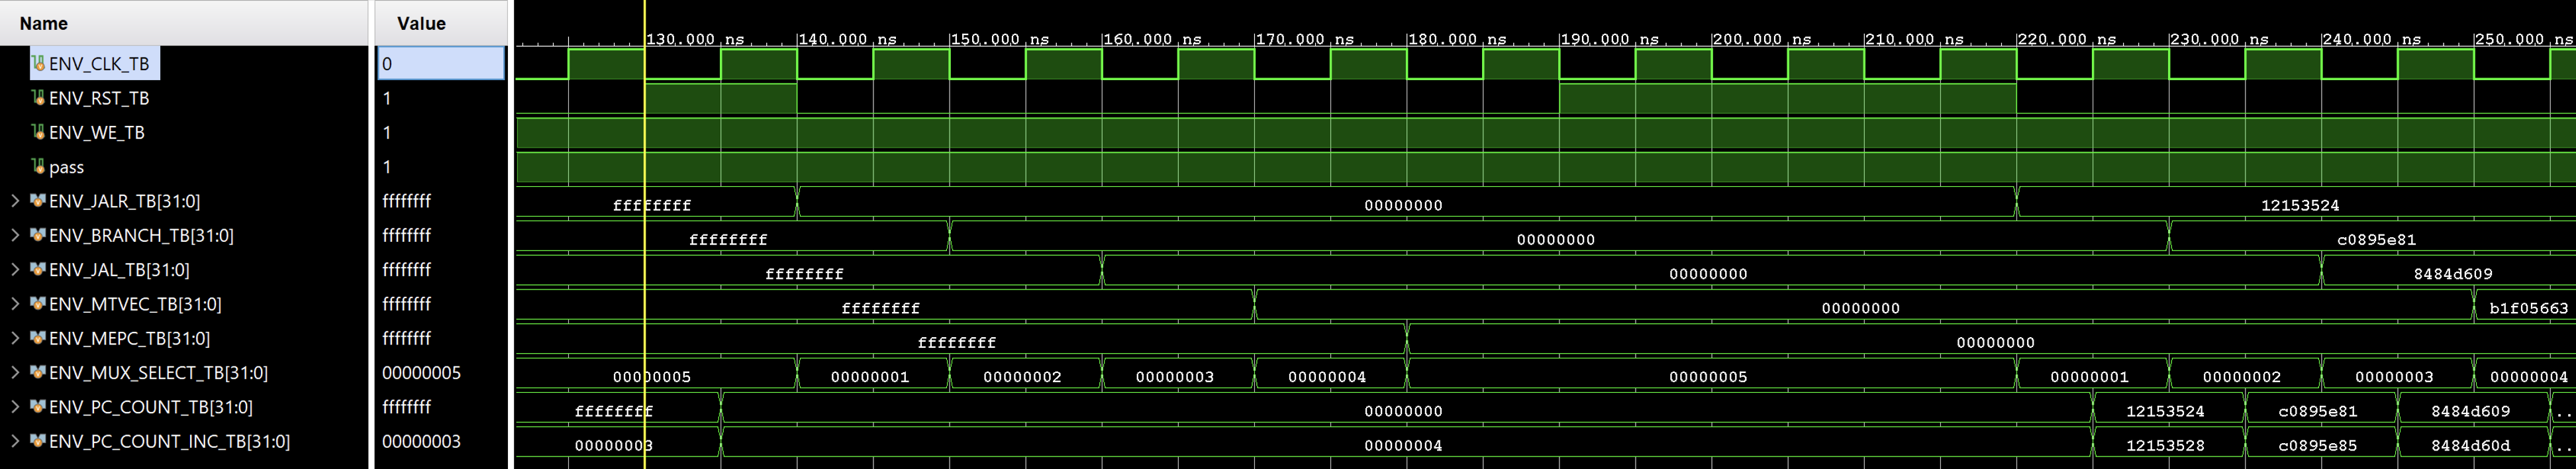
\includegraphics[width=.8\pdfpagewidth]{Figures/Program Counter Simulation 2.png}}
    \caption{Program Counter Simulation 130ns - 250ns}
    \label{fig:PCSimulation}
\end{figure}

\begin{figure}[H]
    \centering
    \captionsetup{style=widetable}
    \makebox[.80\pdfpagewidth]{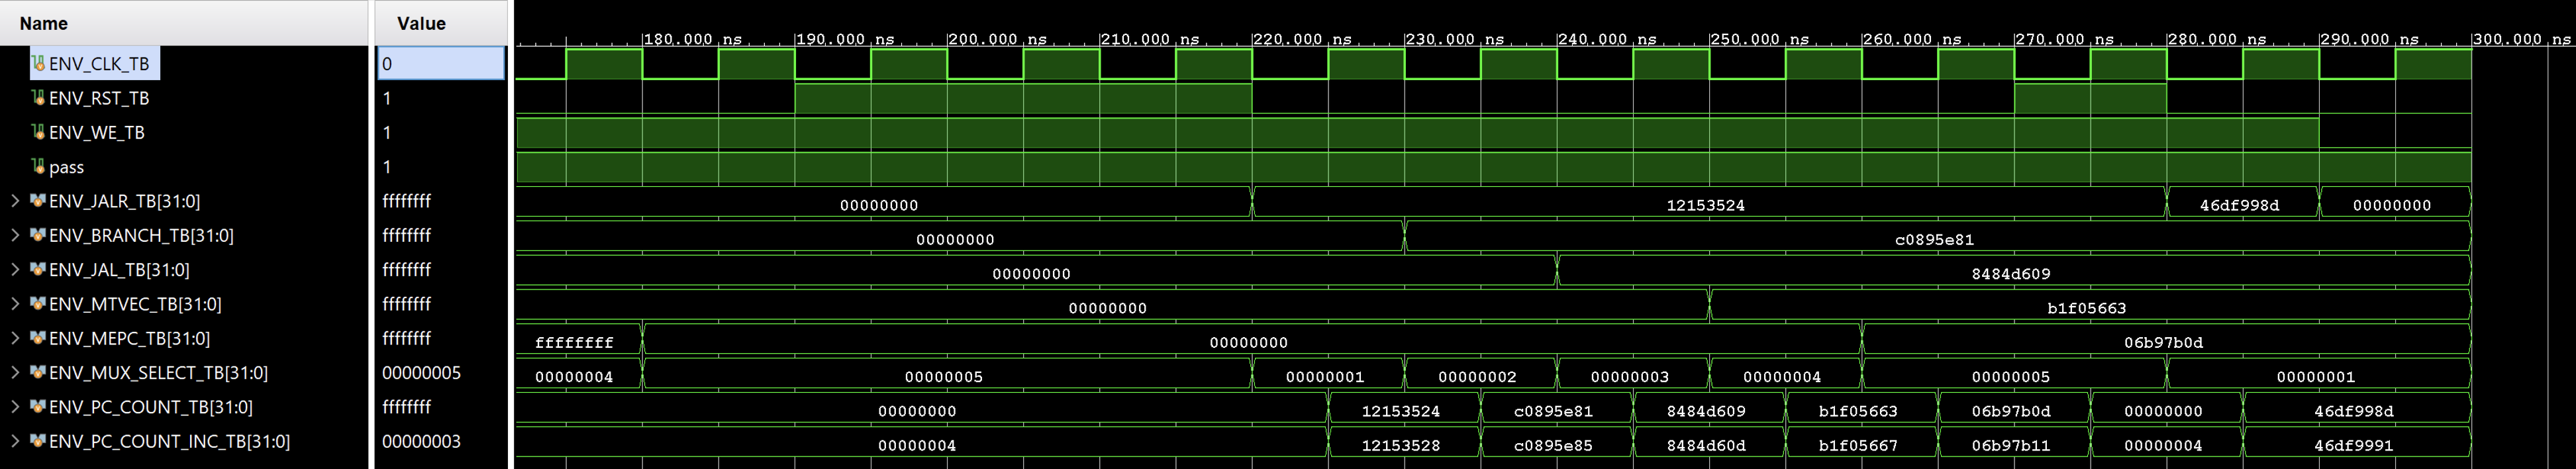
\includegraphics[width=.8\pdfpagewidth]{Figures/Program Counter Simulation 3.png}}
    \caption{Program Counter Simulation 180ns - 300ns}
    \label{fig:PCSimulation}
\end{figure}


\section{Source Code}
\captionsetup{style=widetable}
\subsection{Program Counter} % Third level section

\lstinputlisting[language=Verilog, caption=Verilog Code for Program Counter]{/Users/ethanvosburg/Documents/git/CPE-233-Otter/HW2-ProgramCounter/ProgramCounter/ProgramCounter.srcs/sources_1/new/ProgramCounter.sv}

\subsection{Program Counter Multiplexer} % Third level section

\lstinputlisting[language=Verilog, caption=Verilog Code for Program Counter]{/Users/ethanvosburg/Documents/git/CPE-233-Otter/HW2-ProgramCounter/ProgramCounter/ProgramCounter.srcs/sources_1/new/ProgramCounterMux.sv}

\subsection{Program Counter Environment} % Third level section

\lstinputlisting[language=Verilog, caption=Verilog Code for Program Counter]{/Users/ethanvosburg/Documents/git/CPE-233-Otter/HW2-ProgramCounter/ProgramCounter/ProgramCounter.srcs/sources_1/new/ProgramCounterEnv.sv}



\section {Conclusion} % Second level section
\hypersetup{urlcolor=blue} 
The program counter is a very important module and will be used heavily in the Otter processor. This counter keeps track of which line of machine code to feed the rest of the processor and it makes allows branching and many other capabilities. In this project, a program counter was created and tested using a testbench. The testbench was able to verify that the program counter and the mux associated with it worked properly and passed all of the test cases.
All code for this assignment can be found \href{https://github.com/EthanV1920/CPE-233-Otter/tree/main}{here}.


\end{fullwidth}

% \beg 


%----------------------------------------------------------------------------------------

\end{document}
